% SplitEdgeKey — Embedded property storage layout
\documentclass[tikz,border=4mm]{standalone}
\usepackage[T1]{fontenc}
\usepackage{lmodern}
% Shared TikZ styles for Flexograph table-layout diagrams.
% Include with % Shared TikZ styles for Flexograph table-layout diagrams.
% Include with % Shared TikZ styles for Flexograph table-layout diagrams.
% Include with \input{schema_styles} in each standalone figure.

\usetikzlibrary{shapes.multipart, arrows.meta, positioning, fit, calc, backgrounds}

% ── Colour palette ──────────────────────────────────────────────────
\definecolor{tblheader}{HTML}{2C3E50}   % dark blue-grey header bar
\definecolor{tblbody}{HTML}{ECF0F1}     % light grey table body
\definecolor{sentbg}{HTML}{D5DBDB}      % sentinel row shading
\definecolor{cgTemporal}{HTML}{AED6F1}  % column group: temporal
\definecolor{cgName}{HTML}{A9DFBF}      % column group: name
\definecolor{cgContact}{HTML}{F9E79F}   % column group: contact
\definecolor{cgLocation}{HTML}{F5CBA7}  % column group: location
\definecolor{cgContent}{HTML}{D2B4DE}   % column group: content
\definecolor{structClr}{HTML}{85929E}   % structural table border
\definecolor{propClr}{HTML}{2980B9}     % property table border
\definecolor{secClr}{HTML}{27AE60}      % secondary table border
\definecolor{arrowClr}{HTML}{7F8C8D}    % relationship arrows

% ── Node styles ─────────────────────────────────────────────────────
\tikzset{
  % Table header bar
  tblhdr/.style={
    rectangle, draw=tblheader, fill=tblheader,
    text=white, font=\sffamily\bfseries\footnotesize,
    minimum width=#1, minimum height=5mm, inner sep=2pt,
    align=center,
  },
  tblhdr/.default=38mm,
  % Table body (single cell / row)
  tblcell/.style={
    rectangle, draw=tblheader!40, fill=tblbody,
    font=\sffamily\scriptsize, minimum width=#1,
    minimum height=4.5mm, inner sep=2pt, align=center,
  },
  tblcell/.default=38mm,
  % Sentinel-row variant
  sentcell/.style={
    tblcell=#1, fill=sentbg,
  },
  sentcell/.default=38mm,
  % Column-group cell (coloured)
  cgcell/.style 2 args={
    tblcell=#1, fill=#2,
  },
  % Key column (narrower, left-aligned)
  keycell/.style={
    tblcell=#1, font=\sffamily\scriptsize\itshape,
  },
  keycell/.default=18mm,
  % Format annotation
  fmtlabel/.style={
    font=\sffamily\tiny\color{tblheader!70}, anchor=north west,
  },
  % Dashed grouping box
  groupbox/.style={
    rectangle, rounded corners=2pt, draw=#1, densely dashed,
    line width=0.6pt, inner sep=3pt,
  },
  groupbox/.default=structClr,
  % Relationship arrow
  relarrow/.style={
    -{Stealth[length=2.5mm]}, arrowClr, line width=0.5pt,
  },
  % Label for relationship
  rellabel/.style={
    font=\sffamily\tiny\color{arrowClr}, midway, fill=white, inner sep=1pt,
  },
}
 in each standalone figure.

\usetikzlibrary{shapes.multipart, arrows.meta, positioning, fit, calc, backgrounds}

% ── Colour palette ──────────────────────────────────────────────────
\definecolor{tblheader}{HTML}{2C3E50}   % dark blue-grey header bar
\definecolor{tblbody}{HTML}{ECF0F1}     % light grey table body
\definecolor{sentbg}{HTML}{D5DBDB}      % sentinel row shading
\definecolor{cgTemporal}{HTML}{AED6F1}  % column group: temporal
\definecolor{cgName}{HTML}{A9DFBF}      % column group: name
\definecolor{cgContact}{HTML}{F9E79F}   % column group: contact
\definecolor{cgLocation}{HTML}{F5CBA7}  % column group: location
\definecolor{cgContent}{HTML}{D2B4DE}   % column group: content
\definecolor{structClr}{HTML}{85929E}   % structural table border
\definecolor{propClr}{HTML}{2980B9}     % property table border
\definecolor{secClr}{HTML}{27AE60}      % secondary table border
\definecolor{arrowClr}{HTML}{7F8C8D}    % relationship arrows

% ── Node styles ─────────────────────────────────────────────────────
\tikzset{
  % Table header bar
  tblhdr/.style={
    rectangle, draw=tblheader, fill=tblheader,
    text=white, font=\sffamily\bfseries\footnotesize,
    minimum width=#1, minimum height=5mm, inner sep=2pt,
    align=center,
  },
  tblhdr/.default=38mm,
  % Table body (single cell / row)
  tblcell/.style={
    rectangle, draw=tblheader!40, fill=tblbody,
    font=\sffamily\scriptsize, minimum width=#1,
    minimum height=4.5mm, inner sep=2pt, align=center,
  },
  tblcell/.default=38mm,
  % Sentinel-row variant
  sentcell/.style={
    tblcell=#1, fill=sentbg,
  },
  sentcell/.default=38mm,
  % Column-group cell (coloured)
  cgcell/.style 2 args={
    tblcell=#1, fill=#2,
  },
  % Key column (narrower, left-aligned)
  keycell/.style={
    tblcell=#1, font=\sffamily\scriptsize\itshape,
  },
  keycell/.default=18mm,
  % Format annotation
  fmtlabel/.style={
    font=\sffamily\tiny\color{tblheader!70}, anchor=north west,
  },
  % Dashed grouping box
  groupbox/.style={
    rectangle, rounded corners=2pt, draw=#1, densely dashed,
    line width=0.6pt, inner sep=3pt,
  },
  groupbox/.default=structClr,
  % Relationship arrow
  relarrow/.style={
    -{Stealth[length=2.5mm]}, arrowClr, line width=0.5pt,
  },
  % Label for relationship
  rellabel/.style={
    font=\sffamily\tiny\color{arrowClr}, midway, fill=white, inner sep=1pt,
  },
}
 in each standalone figure.

\usetikzlibrary{shapes.multipart, arrows.meta, positioning, fit, calc, backgrounds}

% ── Colour palette ──────────────────────────────────────────────────
\definecolor{tblheader}{HTML}{2C3E50}   % dark blue-grey header bar
\definecolor{tblbody}{HTML}{ECF0F1}     % light grey table body
\definecolor{sentbg}{HTML}{D5DBDB}      % sentinel row shading
\definecolor{cgTemporal}{HTML}{AED6F1}  % column group: temporal
\definecolor{cgName}{HTML}{A9DFBF}      % column group: name
\definecolor{cgContact}{HTML}{F9E79F}   % column group: contact
\definecolor{cgLocation}{HTML}{F5CBA7}  % column group: location
\definecolor{cgContent}{HTML}{D2B4DE}   % column group: content
\definecolor{structClr}{HTML}{85929E}   % structural table border
\definecolor{propClr}{HTML}{2980B9}     % property table border
\definecolor{secClr}{HTML}{27AE60}      % secondary table border
\definecolor{arrowClr}{HTML}{7F8C8D}    % relationship arrows

% ── Node styles ─────────────────────────────────────────────────────
\tikzset{
  % Table header bar
  tblhdr/.style={
    rectangle, draw=tblheader, fill=tblheader,
    text=white, font=\sffamily\bfseries\footnotesize,
    minimum width=#1, minimum height=5mm, inner sep=2pt,
    align=center,
  },
  tblhdr/.default=38mm,
  % Table body (single cell / row)
  tblcell/.style={
    rectangle, draw=tblheader!40, fill=tblbody,
    font=\sffamily\scriptsize, minimum width=#1,
    minimum height=4.5mm, inner sep=2pt, align=center,
  },
  tblcell/.default=38mm,
  % Sentinel-row variant
  sentcell/.style={
    tblcell=#1, fill=sentbg,
  },
  sentcell/.default=38mm,
  % Column-group cell (coloured)
  cgcell/.style 2 args={
    tblcell=#1, fill=#2,
  },
  % Key column (narrower, left-aligned)
  keycell/.style={
    tblcell=#1, font=\sffamily\scriptsize\itshape,
  },
  keycell/.default=18mm,
  % Format annotation
  fmtlabel/.style={
    font=\sffamily\tiny\color{tblheader!70}, anchor=north west,
  },
  % Dashed grouping box
  groupbox/.style={
    rectangle, rounded corners=2pt, draw=#1, densely dashed,
    line width=0.6pt, inner sep=3pt,
  },
  groupbox/.default=structClr,
  % Relationship arrow
  relarrow/.style={
    -{Stealth[length=2.5mm]}, arrowClr, line width=0.5pt,
  },
  % Label for relationship
  rellabel/.style={
    font=\sffamily\tiny\color{arrowClr}, midway, fill=white, inner sep=1pt,
  },
}


\begin{document}
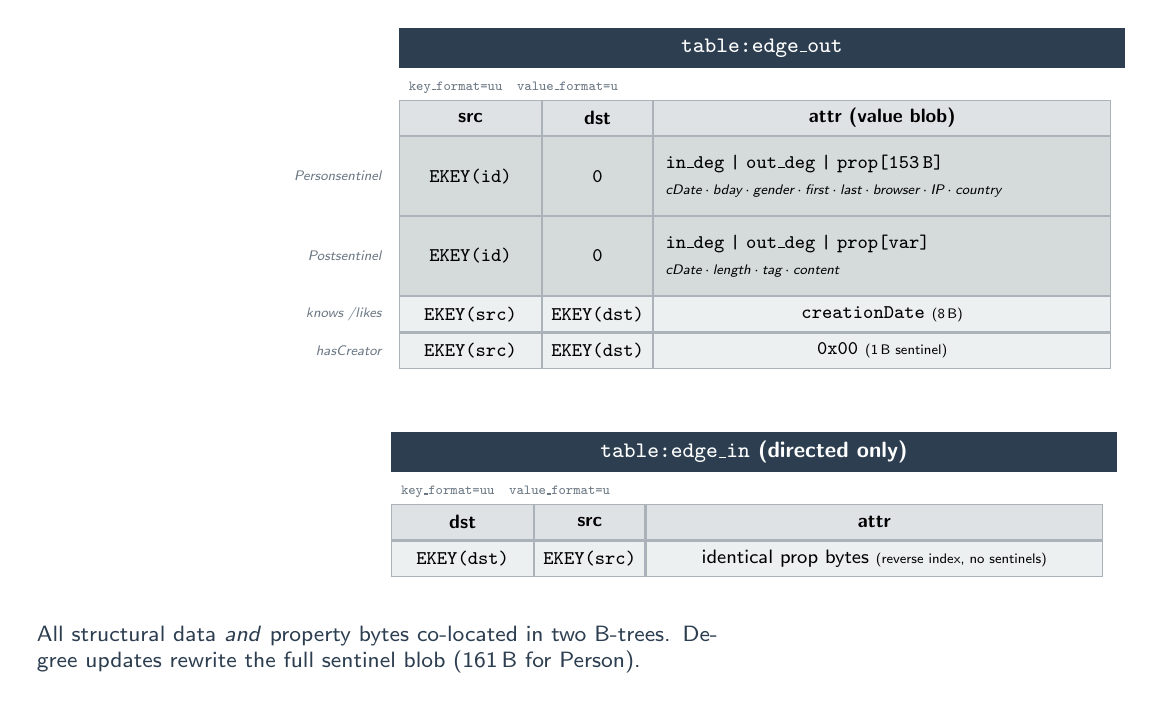
\begin{tikzpicture}[node distance=0mm]

% ════════════════════════════════════════════════════════════════════
%  TABLE: edge_out
% ════════════════════════════════════════════════════════════════════
\node[tblhdr=92mm] (eout-hdr) {\texttt{table:edge\_out}};
\node[fmtlabel, below right=0.5mm and 0mm of eout-hdr.south west]
  (eout-fmt) {\texttt{key\_format=uu\ \ value\_format=u}};

% Column headers
\node[tblcell=18mm, below=4mm of eout-hdr.south west, anchor=north west,
      fill=tblheader!15, font=\sffamily\scriptsize\bfseries] (ch-src) {src};
\node[tblcell=14mm, right=0mm of ch-src,
      fill=tblheader!15, font=\sffamily\scriptsize\bfseries] (ch-dst) {dst};
\node[tblcell=58mm, right=0mm of ch-dst,
      fill=tblheader!15, font=\sffamily\scriptsize\bfseries] (ch-val) {attr (value blob)};

% ── Person sentinel row ─────────────────────────────────────────
\node[sentcell=18mm, below=0mm of ch-src, minimum height=10mm] (r1-src) {\texttt{EKEY(id)}};
\node[sentcell=14mm, right=0mm of r1-src, minimum height=10mm] (r1-dst) {\texttt{0}};
\node[sentcell=58mm, right=0mm of r1-dst, align=left, text width=55mm,
      minimum height=10mm] (r1-val) {%
  \texttt{in\_deg\;|\;out\_deg\;|\;prop[153\,B]}\\[0.5mm]
  {\tiny\itshape cDate\,$\cdot$\,bday\,$\cdot$\,gender\,$\cdot$\,first\,$\cdot$\,last\,$\cdot$\,browser\,$\cdot$\,IP\,$\cdot$\,country}};

% annotation
\node[font=\sffamily\tiny\itshape, text=tblheader!70,
      left=1mm of r1-src.west, anchor=east] {Person\\[-0.5mm]sentinel};

% ── Post sentinel row ───────────────────────────────────────────
\node[sentcell=18mm, below=0mm of r1-src, minimum height=10mm] (r2-src) {\texttt{EKEY(id)}};
\node[sentcell=14mm, right=0mm of r2-src, minimum height=10mm] (r2-dst) {\texttt{0}};
\node[sentcell=58mm, right=0mm of r2-dst, align=left, text width=55mm,
      minimum height=10mm] (r2-val) {%
  \texttt{in\_deg\;|\;out\_deg\;|\;prop[var]}\\[0.5mm]
  {\tiny\itshape cDate\,$\cdot$\,length\,$\cdot$\,tag\,$\cdot$\,content}};

\node[font=\sffamily\tiny\itshape, text=tblheader!70,
      left=1mm of r2-src.west, anchor=east] {Post\\[-0.5mm]sentinel};

% ── Edge row (knows / likes) ────────────────────────────────────
\node[tblcell=18mm, below=0mm of r2-src] (r3-src) {\texttt{EKEY(src)}};
\node[tblcell=14mm, right=0mm of r3-src] (r3-dst) {\texttt{EKEY(dst)}};
\node[tblcell=58mm, right=0mm of r3-dst] (r3-val) {%
  \texttt{creationDate} {\tiny(8\,B)}};

\node[font=\sffamily\tiny\itshape, text=tblheader!70,
      left=1mm of r3-src.west, anchor=east] {knows /\\[-0.5mm]likes};

% ── Edge row (hasCreator — no props) ────────────────────────────
\node[tblcell=18mm, below=0mm of r3-src] (r4-src) {\texttt{EKEY(src)}};
\node[tblcell=14mm, right=0mm of r4-src] (r4-dst) {\texttt{EKEY(dst)}};
\node[tblcell=58mm, right=0mm of r4-dst] (r4-val) {%
  \texttt{0x00} {\tiny(1\,B sentinel)}};

\node[font=\sffamily\tiny\itshape, text=tblheader!70,
      left=1mm of r4-src.west, anchor=east] {hasCreator};

% ════════════════════════════════════════════════════════════════════
%  TABLE: edge_in
% ════════════════════════════════════════════════════════════════════
\node[tblhdr=92mm, below=8mm of r4-src.south west, anchor=north west,
      xshift=-1mm] (ein-hdr) {\texttt{table:edge\_in} {\footnotesize(directed only)}};
\node[fmtlabel, below right=0.5mm and 0mm of ein-hdr.south west]
  {\texttt{key\_format=uu\ \ value\_format=u}};

\node[tblcell=18mm, below=4mm of ein-hdr.south west, anchor=north west,
      fill=tblheader!15, font=\sffamily\scriptsize\bfseries] (ei-ch-dst) {dst};
\node[tblcell=14mm, right=0mm of ei-ch-dst,
      fill=tblheader!15, font=\sffamily\scriptsize\bfseries] (ei-ch-src) {src};
\node[tblcell=58mm, right=0mm of ei-ch-src,
      fill=tblheader!15, font=\sffamily\scriptsize\bfseries] (ei-ch-val) {attr};

\node[tblcell=18mm, below=0mm of ei-ch-dst] (ei-r1-dst) {\texttt{EKEY(dst)}};
\node[tblcell=14mm, right=0mm of ei-r1-dst] (ei-r1-src) {\texttt{EKEY(src)}};
\node[tblcell=58mm, right=0mm of ei-r1-src] (ei-r1-val)
  {identical prop bytes {\tiny(reverse index, no sentinels)}};

% ── Caption ─────────────────────────────────────────────────────
\node[font=\sffamily\footnotesize, text=tblheader, anchor=north west,
      below=5mm of ein-hdr.south west |- ei-r1-dst.south, text width=90mm]
  {All structural data \emph{and} property bytes co-located in two B-trees.
   Degree updates rewrite the full sentinel blob (161\,B for Person).};

\end{tikzpicture}
\end{document}
